\section{Experiments}

\subsection{Dataset Description}
In order to test our itinerary planning system, we used curated sets of Points of Interest (POIs) for seven large cities namely: Delhi, Budapest, Vienna, Osaka, Glasgow, Edinburgh, and Perth. The initial dataset utilized is derived from the \textbf{Yahoo Flickr Creative Commons 100 Million Dataset (YFCC100M)} \cite{}, containing over 100 million images, of which 69 million are annotated and 48 million are geotagged. \ab{69+48>100}

We used the Flickr User-POI Visits dataset available at ~\cite{limkwanhuiDataCode}, \ab{are we using 2 separate datasets?} which was generated in the following manner. In order to generate this dataset, the authors of the paper ~\cite{taylor2018tour} took a set of popular POIs for every city mentioned earlier using resources such as \textit{Wikipedia}. Then, geotagged photos in \textit{Flickr} were matched with these POIs using spatial proximity. By estimating relative \textbf{popularity} of a POI through the counts of photos for every POI, the relative popularity which is referred to as utility was estimated.

This approach generates an empirical proxy for real tourist behavior, measuring interest in a specific attraction as measured by publicly accessible, crowd-sourced images.

The existing dataset contained the following key fields for each POI:

\begin{table}[H]
\begin{tabularx}{0.5\textwidth}{p{3cm} X}
\hline
\textbf{Field Name} & \textbf{Description} \\
\hline
\texttt{poiID} & A unique identifier assigned to each POI. \\
\hline
\texttt{poiName} & The name of the POI, e.g., ``Red Fort'', ``Osaka Castle''. \\
\hline
\texttt{lat} & Latitude coordinate of the POI. \\
\hline
\texttt{long} & Longitude coordinate of the POI. \\
\hline
\texttt{theme or category} & Thematic classification of the POI, such as \textit{amusement}, \textit{historical}, \textit{museum}, \textit{shopping}, \textit{park}, etc. \\
\hline
\texttt{Utility Score or Profit} & A numerical value representing the estimated utility or attractiveness of the POI, derived based on its popularity (photo frequency). \\
\hline
\texttt{Cost} & Geospatial travel distance (in meters) between pairs of POIs. This is used in the travel time estimation between locations, with the walking speed $v_w$ and taxi speed $v_t$. \\
\hline
\end{tabularx}
\caption{Original dataset fields}
\end{table}

\subsection{Experimental Setup}

With an aim to make our system more realistic and practical to use, we supplemented the dataset manually with real-life operating limitations and data that we gathered from \textbf{official tourist websites} and verified online portals. The added fields are:

\begin{table}[H]
\centering
\begin{tabularx}{0.5\textwidth}{p{3cm} X}
\toprule
\textbf{Field Name} & \textbf{Description} \\
\midrule
\texttt{fees} & Entrance fee or ticket price associated with the POI, in INR. \\
\midrule
\texttt{opening time} & The time at which the POI opens for visitors, stored in \texttt{HH:MM:SS} format. \\
\midrule
\texttt{closing time} & The time at which the POI closes for visitors, stored similarly. \\
\midrule
\texttt{Days of Week} & Seven binary columns (\texttt{Monday}, \texttt{Tuesday}, ..., \texttt{Sunday}). A value of 1 indicates the POI is open on that day; 0 indicates it is closed. \\
\midrule
\texttt{Avg Visiting Time} & The average duration (in minutes) tourists typically spend at the POI. \\
\bottomrule
\end{tabularx}
\caption{Additional features added to the dataset}
\end{table}

These manually extracted features add a \textbf{temporal and availability aspect} to the optimisation problem, allowing more realistic and accurate itinerary generation. For example, POIs closed on the chosen day are excluded from the planning automatically.

All the other information was collected by scraping or quoting \textbf{official tourist boards}, \textbf{city tourism websites}, and trustworthy travel websites.

\subsection{Configuration}

The experiments were conducted on a MacBook Air equipped with an Apple M1 processor and 8GB of RAM, providing a lightweight yet efficient environment for developing and testing the itinerary planning system. The implementation was carried out in Python, leveraging its rich ecosystem for data handling, user interaction, and visualization. The core optimization process was performed using the Gurobi Optimizer, a state-of-the-art solver for mathematical programming. Gurobi was employed to solve the underlying Integer Linear Programming (ILP) formulations that generate optimized multi-day travel itineraries under various user-defined constraints and real-world conditions.

\subsection{Baseline Itinerary Planner}

To establish a baseline for evaluation, we implemented the itinerary planning model described in Taylor and Lim \cite{taylor2018tour}, which we refer to as the \textbf{baseline model}. This model adopts a binary decision framework, where each Point of Interest (POI) is either fully included in the itinerary or completely excluded. The utility function in this setting is defined as:

\[
\max \left\{ \sum_{i=2}^{N} \sum_{j=2}^{N} S_i \cdot x_{i,j} \right\}
\]

, where \( x_{i,j} = 1 \) if POI \( i \) is visited immediately before POI \( j \), and 0 otherwise. \ab{what is $s_i$?} This is equivalent to the binary utility formulation:

\[
\sum_{i=1}^{N} U(v_i) \cdot y_i
\]

where \( U(v_i) \) denotes the utility of POI \( v_i \), and \( y_i \in \{0,1\} \) is a binary variable indicating whether \( v_i \) is selected in the itinerary.

The baseline model incorporates only fundamental constraints, including the time budget constraint, connectivity requirements, a restriction preventing a direct path between the start and the end POIs, and  sub-tour elimination constraints. In our implementation, the sub-tour elimination is effectively enforced using arrival-time-based constraints. We were able to seamlessly adapt our ILP-based framework to replicate this baseline behavior, effectively converting our advanced planner into a simplified version matching the baseline model's structure.

However, direct performance comparison between our model and the baseline was not feasible due to a key limitation in the common dataset used by both our system and Taylor and Lim \cite{taylor2018tour} --namely, the absence of standardized POI visiting durations. Second, the baseline paper distributed POI visit durations by an unspecified method, making it impossible to reproduce exactly the same execution cases. Despite this, we were able to re-implement the baseline model in its entirety in terms of constraints as well as utility structure, which provided a good basis for qualitative analysis. \ab{No mention of absence of cost budget}

\subsection{9 Variants of the \trip}

We evaluate the performance of the \trip solution by considering its variants as listed in Table~\ref{tab:trip_variants}, that are based on the transportation mode and the chosen utility variant. 
\begin{table}[H]
\centering
\begin{tabular}{|l|l|l|}
\hline
\textbf{TRIP VARIANT} & \textbf{Transportation Mode} & \textbf{Utility Variant} \\
\hline
TRIP\_W\_B & Walk & Binary \\
TRIP\_T\_B & Taxi & Binary \\
TRIP\_H\_B & Hybrid -- Walk + Taxi & Binary \\
TRIP\_W\_C & Walk & Fractional -- CLF \\
TRIP\_T\_C & Taxi & Fractional -- CLF \\
TRIP\_H\_C & Hybrid -- Walk + Taxi & Fractional -- CLF \\
TRIP\_W\_M & Walk & Fractional -- Slabs \\
TRIP\_T\_M & Taxi & Fractional -- Slabs \\
TRIP\_H\_M & Hybrid -- Walk + Taxi & Fractional -- Slabs \\
\hline
\end{tabular}
\caption{\trip Variants by Transportation Mode and Utility Variant}
\label{tab:trip_variants}
\end{table}


\subsection{Input Parameters and Performance Metrics}

\textbf{User Inputs}\\
Our trip planning system is capable of accepting a wide range of user inputs to support personalized and realistic trip planning. They are:

\begin{itemize}
    \item \textbf{City Choice:} The city would be selected by the user from options.
    
    \item \textbf{Trip Day:} The actual day on which the trip is to take place.

    \item \textbf{Start and End Points:} Latitude and longitude coordinates identifying the point where the day's journey begins and ends.
    
    \item \textbf{User Preferences:}
    \begin{itemize}
        \item \textbf{Category Constraints:} Limit on the category of POIs to be addressed, i.e., museum, market, park, etc.
        \item \textbf{Must-See and Must-Exclude POIs:} Individual POIs that the user must add or remove from the itinerary.
        \item \textbf{Ordering Constraints:} Ordering constraints with respect to POIs, indicating visit priority.
    \end{itemize}
    
	\item Utility Variant: \ab{Add the utility variants}
    \item \textbf{Time Budget:} The time (minutes or hours) the user is willing to spend on the trip.
    \item \textbf{Cost Budget:} The maximum cost which the user will incur on travel expenditure (e.g., taxi fares) and entry fees of POIs.
    
    \item \textbf{Dynamic Variant Specific Inputs:}
    \begin{itemize}
        \item \textbf{Actual Visitation Time per POI:} Used to update the remaining itinerary dynamically during execution.
        \item \textbf{Actual Travel Time between POIs:} Used to dynamically recalculate transitions and reschedule the visits accordingly.
    \end{itemize}
    
    \item \textbf{Multi-day Trip Specific Inputs:}
    \begin{itemize}
        \item \textbf{Number of Days:} Total number of days in the trip.
        \item \textbf{Start, End, and Hotel Coordinates:} Coordinates specifying the start, end, and overnight locations for each day.
        \item \textbf{Start, End, and Hotel Coordinates:} Coordinates that show the start, end, and overnight locations for every day.
        \item \textbf{Start Time \& Time Budget per Day:} Daily starting time and allowed time budget for each day, \\specified per day (first/last/intermediate day).
    \end{itemize}
\end{itemize}
\vspace{0.5cm}
\noindent\textbf{Performance Metrics}\\
We evaluate the quality and efficiency of the generated itineraries using the following performance metrics:

\begin{itemize}
    \item \textbf{Utility:} The total utility obtained from the selected POIs in the itinerary. It reflects how well the chosen points align with user preferences.
    
    \item \textbf{Running Time:} The time (in seconds) required by the system to compute the itinerary. It is an indicator of the system's computational efficiency.
    
    \item \textbf{Time Utilisation:} The percentage of the user-provided time budget that is actually used in the itinerary:
    \[
    \text{Time Utilisation \%} = \frac{\text{Total time used}}{\text{Time budget}} \times 100
    \]
    
    \item \textbf{Fraction of Time Spent in Travel and Visits:}
    \begin{itemize}
        \item \textbf{Travel Time Fraction:} Ratio of time spent traveling between POIs to the total available time.
        \item \textbf{Visit Time Fraction:} Ratio of time spent visiting POIs to the total available time.
    \end{itemize}
\end{itemize}

\ab{Add Cost Utilization}

These metrics serve as the basis for the comparative analysis and graphical illustrations presented in the subsequent section.

\subsection{Demonstrations}

To demonstrate the performance and insights of our itinerary planning system, we begin with a comprehensive visualization in Figure~\ref{fig:cities}, which presents the variation of utility across different time and cost budgets for all seven cities in our dataset. This offers a broad perspective on how the system adapts to varying resource constraints in diverse urban environments. For the remainder of the analysis, we focus on the city of Osaka as a representative case. Unless stated otherwise, the default time budget is varied within a practical range of 480 to 600 minutes, and the cost budget is chosen to be appropriately aligned with the economic characteristics of the city. This approach allows us to maintain clarity while drawing generalizable conclusions from representative trends observed in one city.

\newpage
\noindent \textbf{Comparison of Multi-day trip in 9 variants with the Baseline Model}
\begin{figure}[H]
\centering
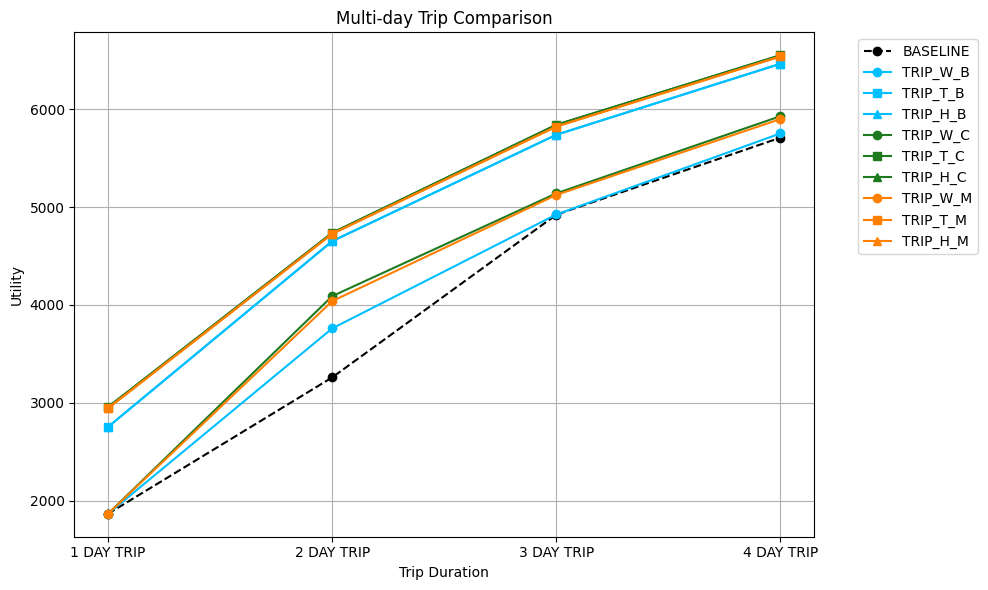
\includegraphics[width=0.4\textwidth]{plots/baselineComparison.png}
\caption{Comparison with Baseline Model}
\label{fig:comparisonWithBaselinePlot}
\end{figure}

The plot~\ref{fig:comparisonWithBaselinePlot} compares the performance of our proposed trip planning variants against a baseline model for trips ranging from one to four days. For a fair comparison, the time budget was fixed at 8 hours per day, and the cost budget was set high at 1,00,000 units - ensuring that cost wouldn’t be a limiting factor, especially for the baseline. The baseline utilities were calculated by creating daily itineraries one after another, making sure not to repeat any POIs from previous days, and summing up the utilities. On the other hand, the nine other variants represent results from our optimized multi-day planning models, which take a more holistic approach. As seen in the graph, all of our variants consistently outperform the baseline across all durations. Given this clear advantage, we have chosen to leave the baseline out of future comparisons to keep things focused. Moreover, this setup results in identical utility values for taxi and hybrid modes, as taxi usage becomes universally optimal due to its time-saving advantage when cost is not an issue. \\

\noindent\textbf{Effect of Multi-modality}

\begin{figure}[H]
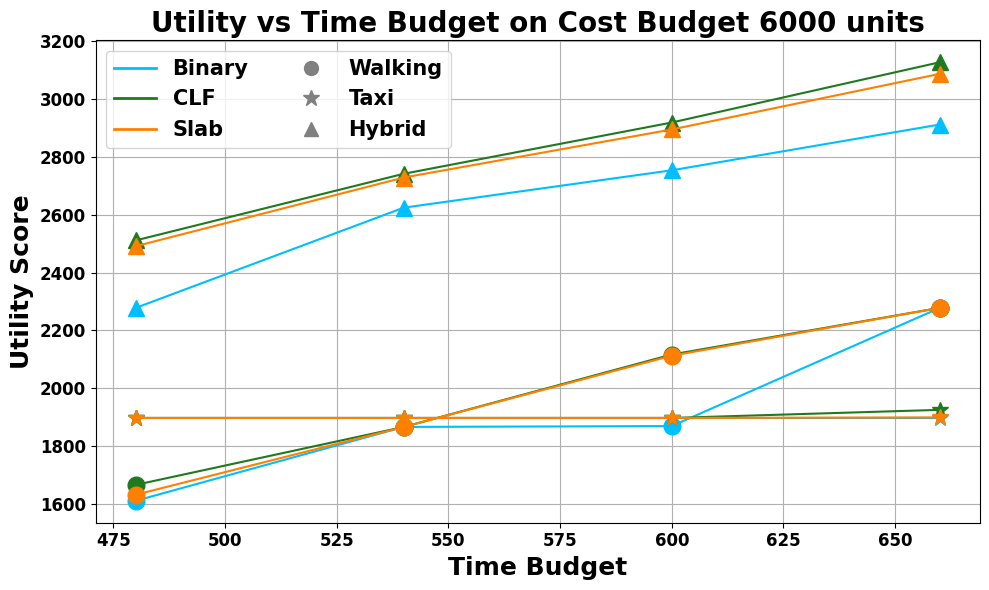
\includegraphics[width=0.4\textwidth]{plots/multimodality1.png}
\label{fig:mm1}
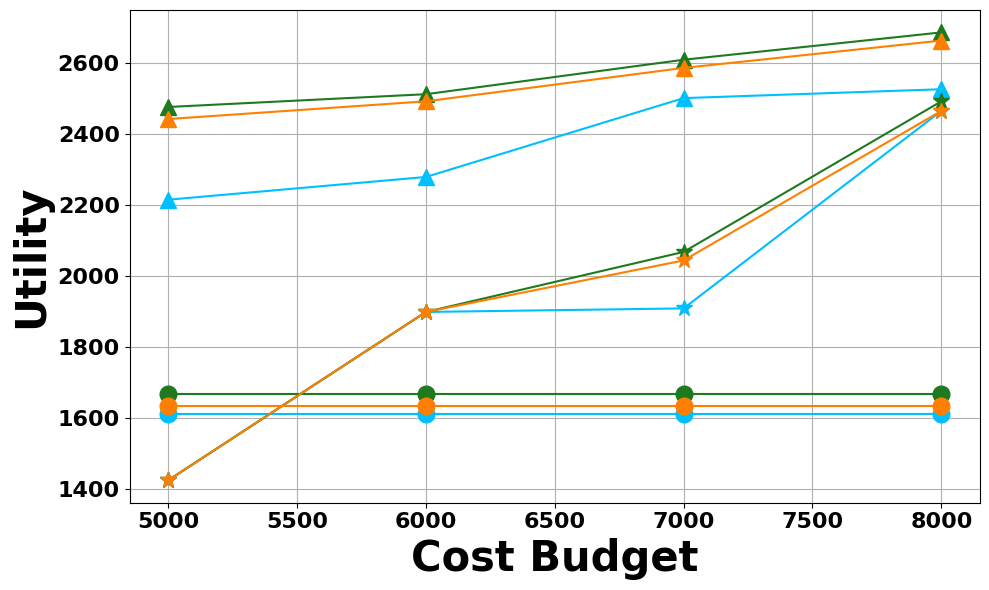
\includegraphics[width=0.4\textwidth]{plots/multimodality2.png}
\caption{Variation of Utility in single-day trips in 9 variants}
\label{fig:mm2}
\end{figure}

Figure ~\ref{fig:mm2} illustrate the impact of varying time and cost budgets on the utility achieved by different transportation modes in our itinerary planning framework. The top graph explores how increasing the time budget (with a fixed cost budget of 6000 units) affects utility. Here, we observe that the utility continues to increase for walking and hybrid modes, while it saturates for the taxi-only variant. This is because the taxi mode relies heavily on cost availability—once the fixed cost budget is consumed, additional time offers very little, to no further improvement. In contrast, the hybrid mode, which leverages both walking and taxi flexibly, consistently outperforms the single-mode options across all three TRIP variants, highlighting the effectiveness of our multi-modality feature.

The lower graph, which holds the time budget constant at 480 minutes while increasing the cost budget, further supports this observation: hybrid models adapt more efficiently to increased resource availability, maximizing utility better than single-mode approaches. In this case, the utility for walking-only variants remains saturated across all TRIP variants, as the potential gains from walking are constrained by the fixed time rather than by cost. Furthermore, a consistent trend is observed wherein the CLF (Continuous Linear Function) scoring model outperforms the slab-based model. This is because CLF assigns utility proportionally to the time spent at a POI—for example, visiting a POI for 63\% of its average duration yields 63\% utility—while the slab model would round this down to 60\% based on predefined thresholds, resulting in a measurable loss. Together, both graphs validate our design choices, demonstrating the combined advantages of multi-modal transportation and continuous utility modeling in enhancing itinerary quality.

\noindent\textbf{Time Utilization}

\begin{figure}[H]
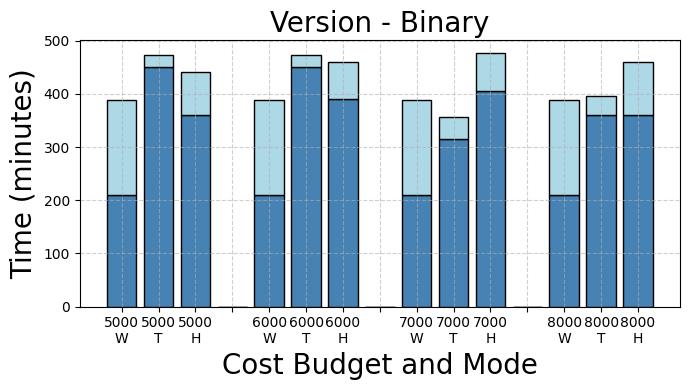
\includegraphics[width=0.23\textwidth]{plots/TIME_UTILIZATION_BINARY.png}
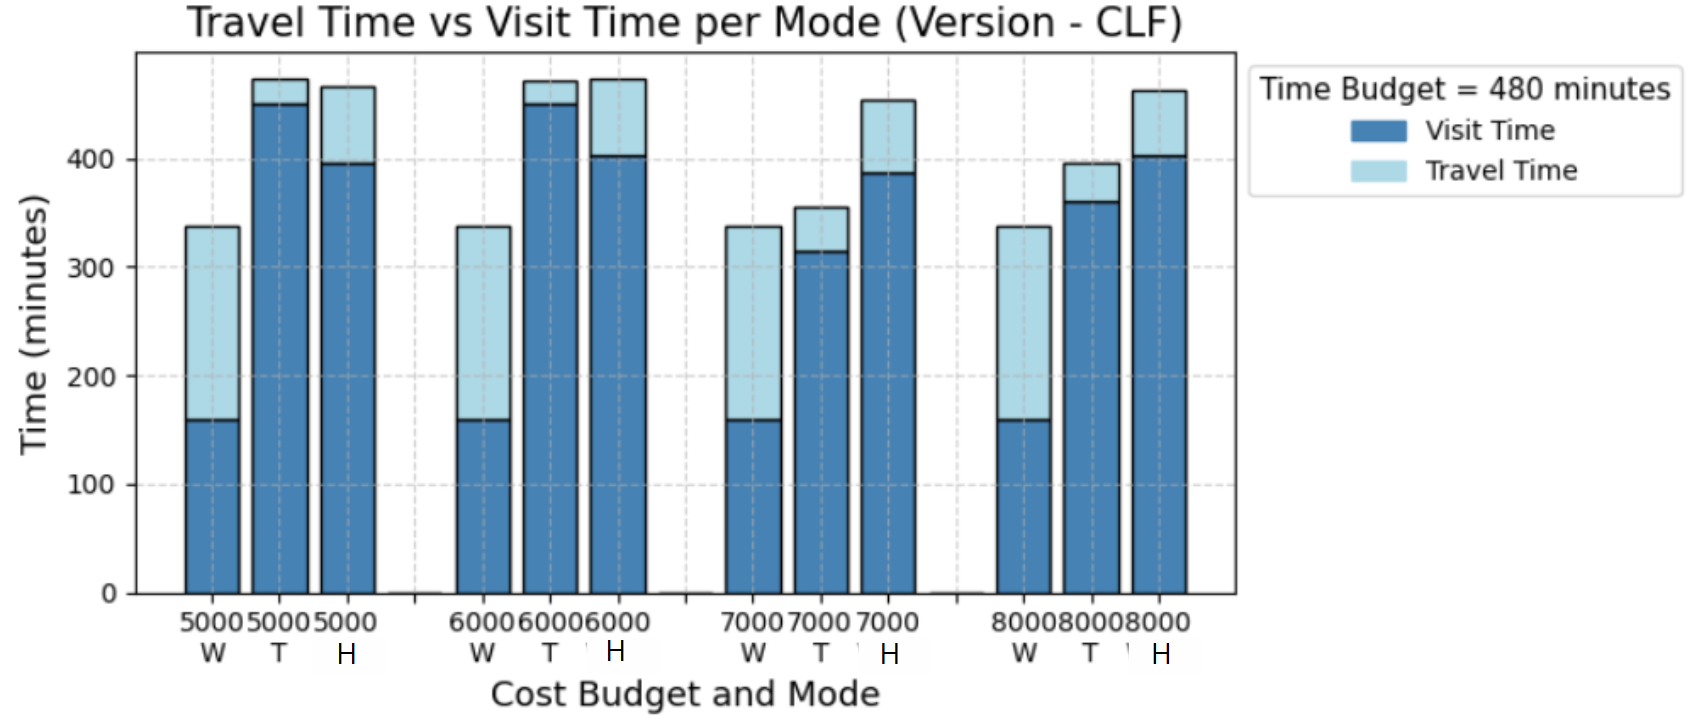
\includegraphics[width=0.23\textwidth]{plots/TIME_UTILIZATION_CLF.png}
\centering
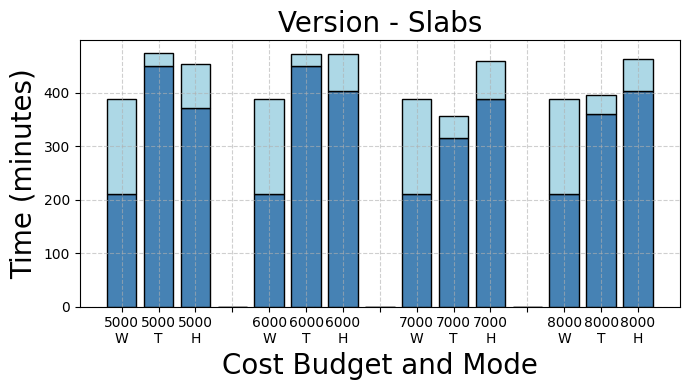
\includegraphics[width=0.23\textwidth]{plots/TIME_UTILIZATION_SLABS.png}
\caption{Time Utilization in 3 Modes- Osaka}
\label{fig:TimeUtilization}
\end{figure}

Figure~\ref{fig:TimeUtilization} presents a comparison of travel time versus visit time across the three TRIP variants---walking-only (TRIP\_W), taxi-only (TRIP\_T), and hybrid (TRIP\_H)---at a fixed time budget of 480 minutes and varying cost budgets (5000, 6000, 7000, and 8000 units). Across all three utility scoring versions (B, C, and M), a clear trend emerges: TRIP\_W exhibits a high travel-to-visit time ratio, reflecting the slower nature of walking as a mode of transport. In contrast, TRIP\_T minimizes travel time due to exclusive reliance on taxis, thereby maximizing time spent at points of interest (POIs). The hybrid model, TRIP\_H, maintains a balanced ratio between travel and visit time, offering a compromise between the two extremes. While the taxi-only model may seem efficient in terms of maximizing visit time, earlier experiments have demonstrated that it is the hybrid TRIP\_H that achieves the highest overall utility. This highlights that optimizing for utility involves not just maximizing visit duration but also strategically balancing travel efficiency with multi-modal flexibility.\\

\noindent\textbf{Utility vs Time budget on different cost budgets}

\begin{figure}[H]
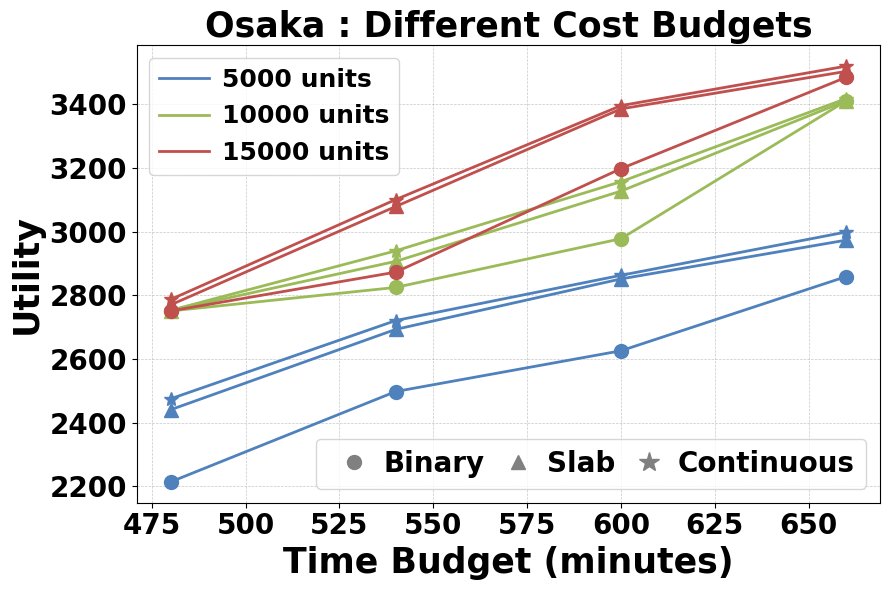
\includegraphics[width=0.22\textwidth]{plots/exp1-osaka.png}
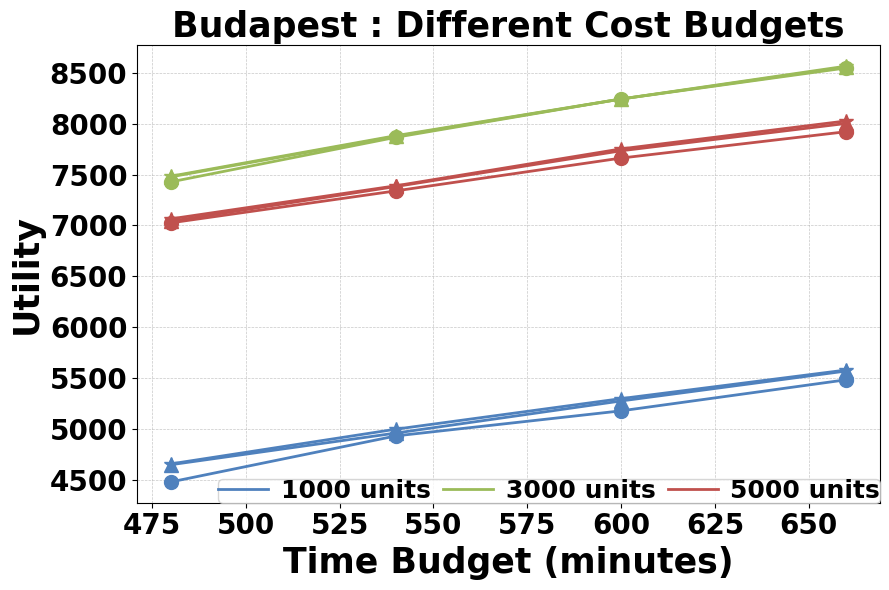
\includegraphics[width=0.22\textwidth]{plots/exp1-budapest.png}
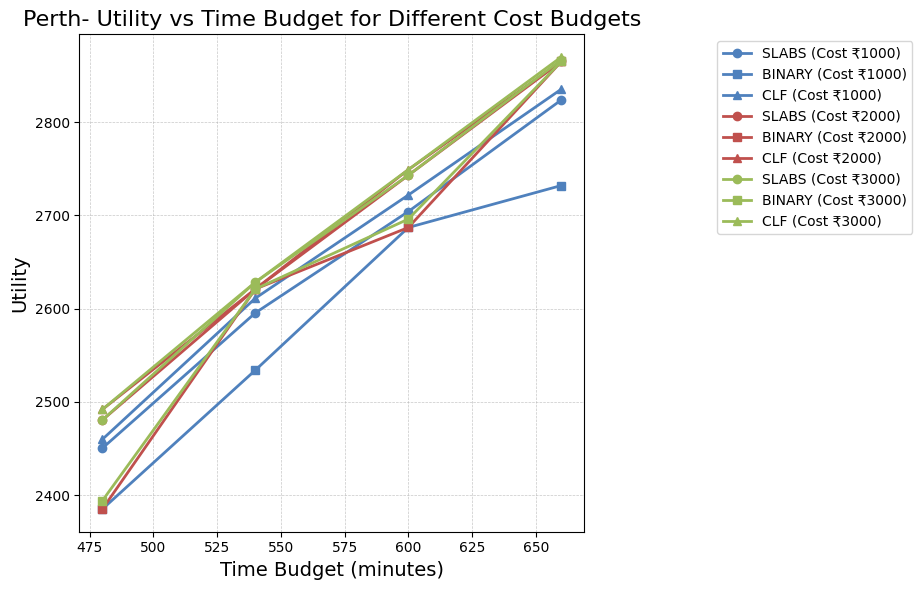
\includegraphics[width=0.22\textwidth]{plots/exp1-perth.png}
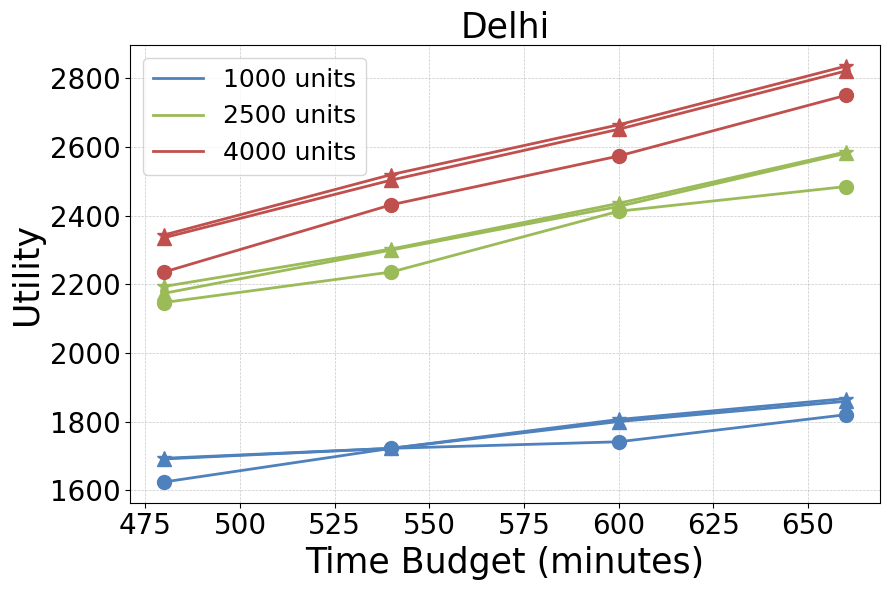
\includegraphics[width=0.22\textwidth]{plots/exp1-delhi.png}
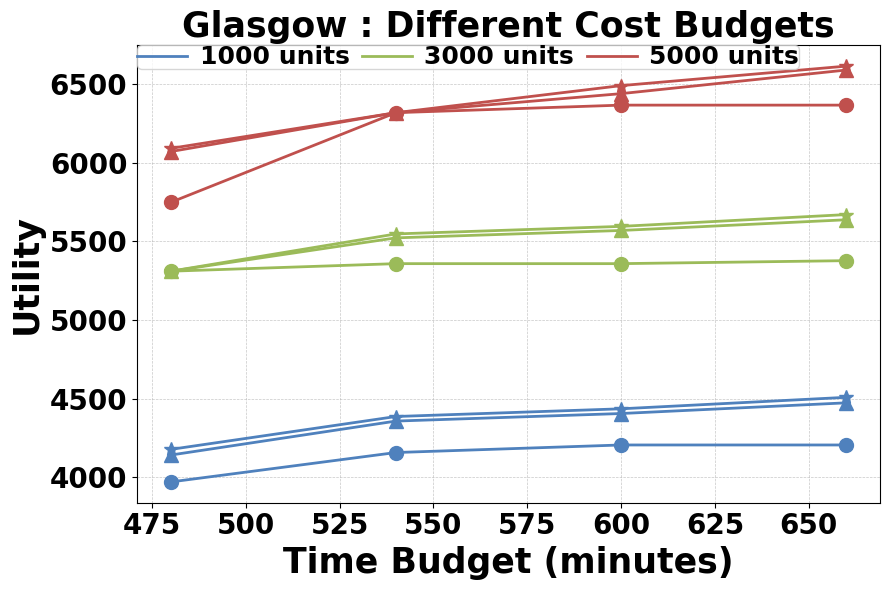
\includegraphics[width=0.22\textwidth]{plots/exp1-glasgow.png}
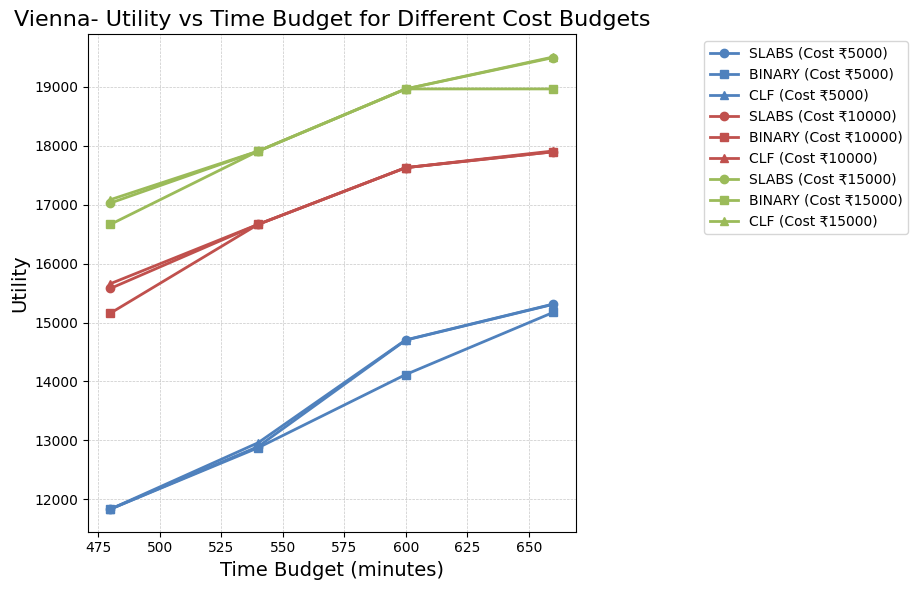
\includegraphics[width=0.22\textwidth]{plots/exp-1 vienna.png}
\centering
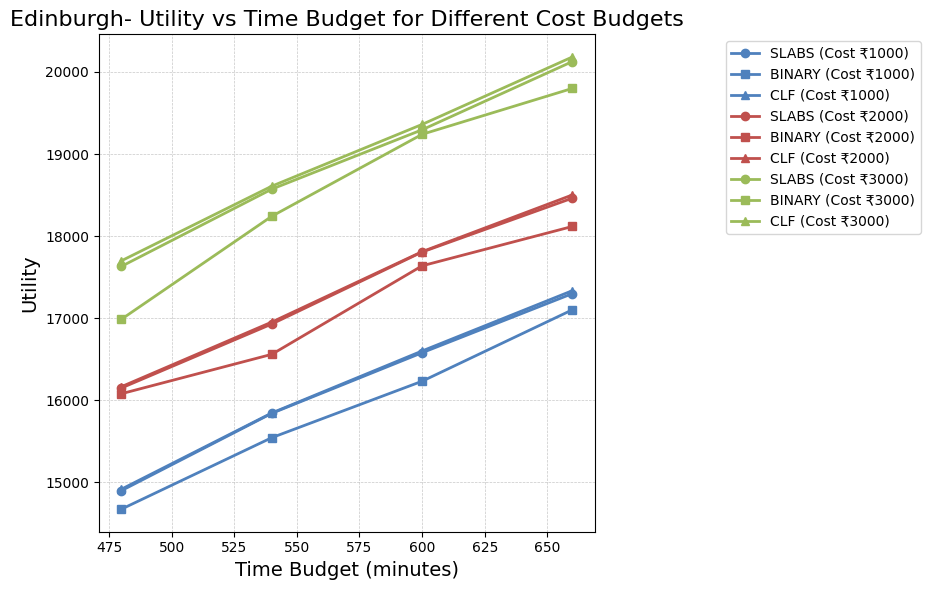
\includegraphics[width=0.22\textwidth]{plots/exp1-edinburgh.png}
\caption{Utility variation with time and cost in 7 cities}
\label{fig:cities}
\end{figure}

Figure~\ref{fig:cities} illustrates how the achieved utility varies across different combinations of time and cost budgets for the seven cities in our dataset. In each plot, line colors represent distinct cost budgets, the X-axis corresponds to increasing time budgets, and marker shapes denote different optimization variants (B, M, and C). A few consistent trends emerge across all cities. First, for a fixed cost budget, increasing the available time consistently leads to higher utility, highlighting the value of longer exploration durations. Second, for a given time budget, allocating a higher cost budget also results in improved utility, indicating the benefit of greater financial flexibility. Most notably, the C variant consistently outperforms both the M and B versions in terms of utility achieved, suggesting its superior effectiveness in balancing constraints across diverse urban scenarios.\\

\newpage
\noindent\textbf{Variation of Utility in Multi-day Itineraries}

\begin{figure}[H]
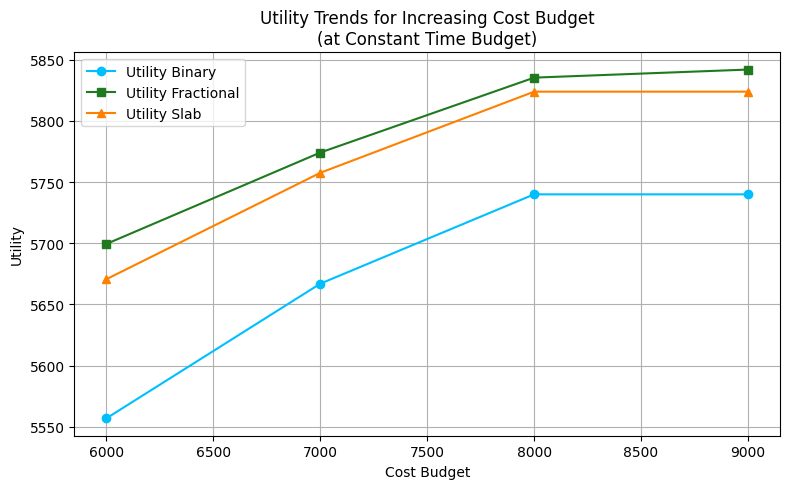
\includegraphics[width=0.22\textwidth]{plots/multiday1.png}
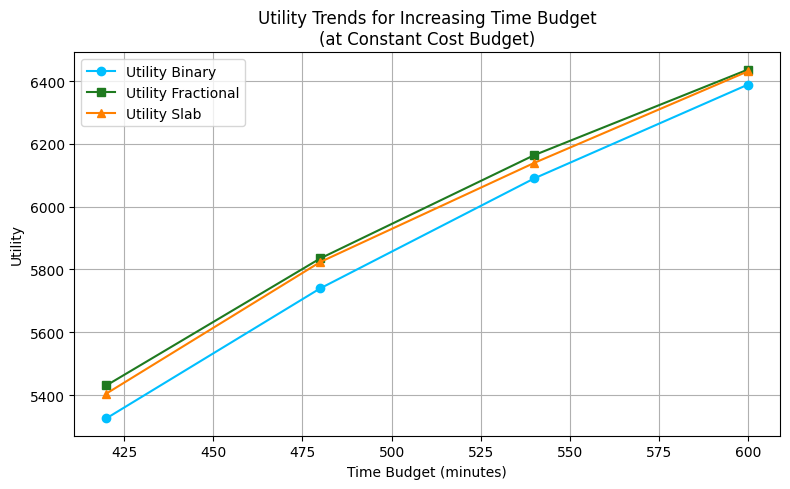
\includegraphics[width=0.22\textwidth]{plots/multiday2.png}
\caption{Trends in Multi-day itineraries}
\label{fig:util_md}
\end{figure}

Figure ~\ref{fig:util_md} presents the utility trends for the multi-day variant of our itinerary planner. Similar to the single-day analysis, a consistent increasing trend in utility results is observed with fixed cost budget and increasing time budget and vice-versa, across the various formulations. Specifically, the utility achieved using the fractional variant is consistently higher than that of the binary variant, reaffirming the advantages of allowing partial visitations in enhancing overall experience. Furthermore, within the fractional formulations, the CLF (Continuous Linear Fractional) approach typically yields higher utility than the slab-based version, demonstrating its stronger capability to balance constraints and exploit budget flexibility effectively across multiple days of planning.\\

\noindent\textbf{Multi-day Trips vs 2 single day trips}
\begin{figure}[H]
\centering
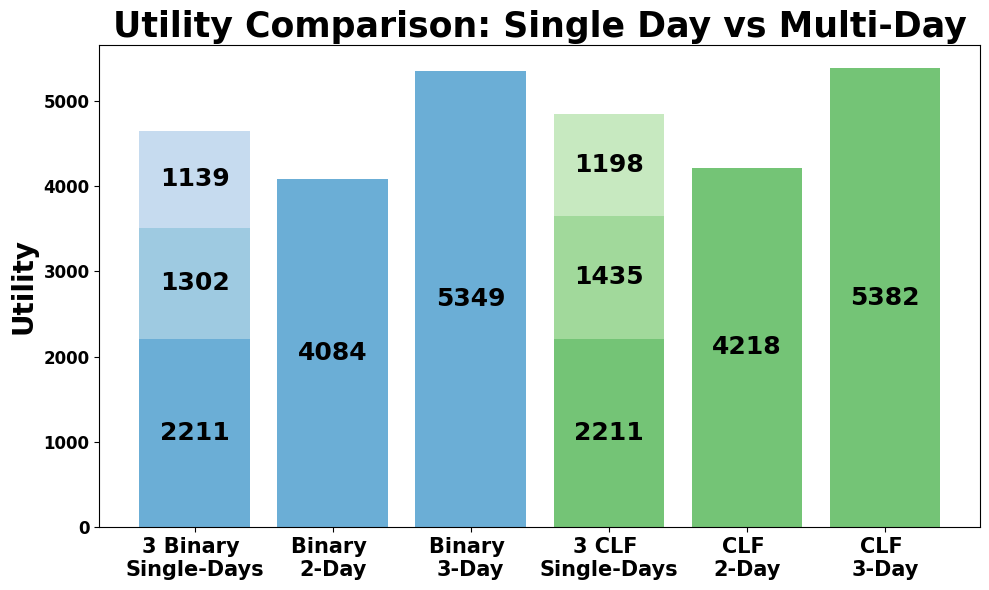
\includegraphics[width=0.5\textwidth]{plots/multivssingle.png}
\caption{Comparison of agreggated Single day trips with 1 multi-day trip}
\label{fig:singlevsmultiday}
\end{figure}
Figure ~\ref{fig:singlevsmultiday} clearly shows that a multi-day trip offers more than just the sum of individual single-day trips. In our experiment, we combined two separate single-day trips, where on the second day, the POIs of first day were extended and compared their total utility with that of a single two-day trip using the multi-day variant. The results were consistent across all three utility measures—Binary, CLF, and Slabs—with the multi-day version yielding noticeably higher utility in each case. This suggests that the multi-day model captures cross-day interactions or efficiencies that are missed when treating each day independently, highlighting the added value of modeling trips across multiple days as a single unit.\\

\noindent\textbf{Effect of personalized constraints}
\begin{figure}[H]
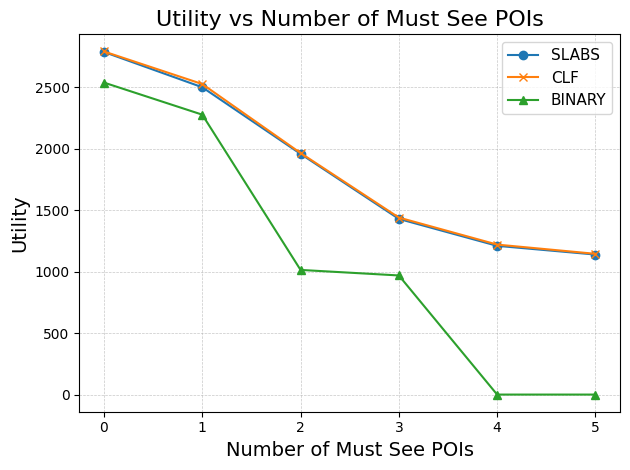
\includegraphics[width=0.23\textwidth]{plots/mustsee.png}
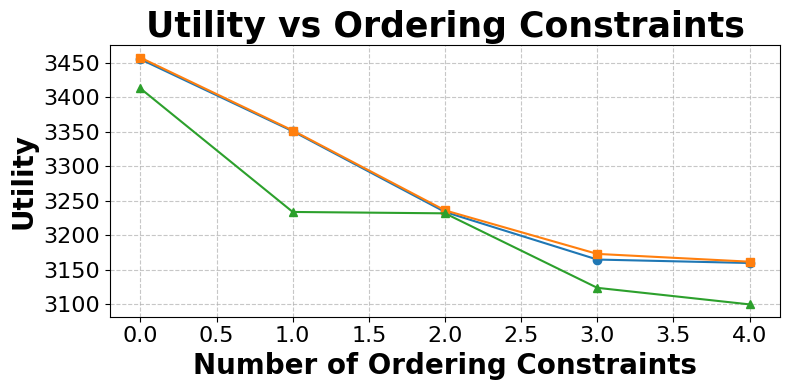
\includegraphics[width=0.23\textwidth]{plots/ordering.png}
\centering
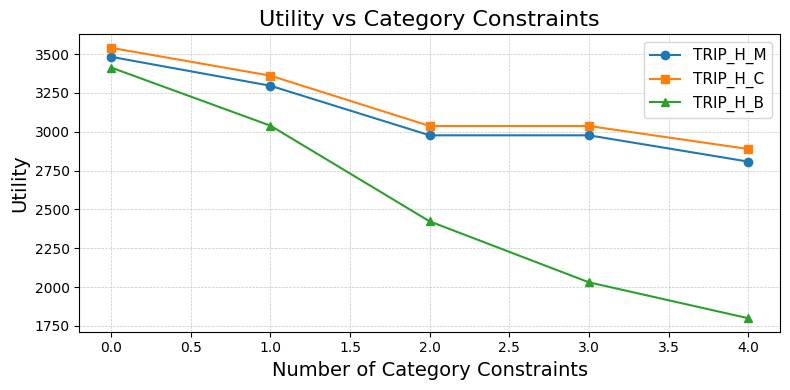
\includegraphics[width=0.23\textwidth]{plots/category.png}
\caption{Effect of Must-see, ordering and category constraints}
\label{fig:personalizedconstraints}
\end{figure}

The impact of incorporating personalized constraints, that is, must-see, ordering, and category constraints, on overall utility is illustrated in the three graphs in figure ~\ref{fig:personalizedconstraints}. Across all cases, it is evident that increasing the number of constraints leads to a decline in the achievable utility, as the solution space becomes more restricted. However, the extent of this reduction varies across the different formulations. Specifically, the CLF and slab variants show a relatively gradual decline in utility compared to the binary variant. This is primarily because the binary model lacks the flexibility to accommodate partial visits to points of interest (POIs), thereby limiting its ability to adapt to tighter constraints. In contrast, the CLF and slab variants can better navigate these constraints by leveraging their ability to assign fractional or grouped visits, thus preserving higher utility under increasingly personalized user preferences.\\

\noindent\textbf{Effect of Dynamic Re-routing}
\begin{figure}[H]
    \centering
    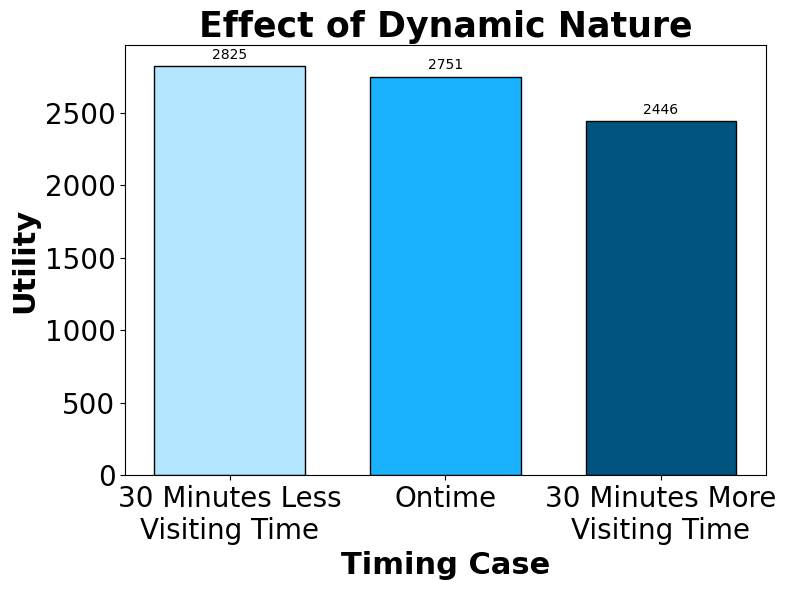
\includegraphics[width=0.25\textwidth]{plots/dynamic.png}
    \caption{Comparison of utility when tourist gets delayed, reaches on time and arrives early}
    \label{fig:dynamic}
\end{figure}

\begin{figure*}[htbp]
    \centering
    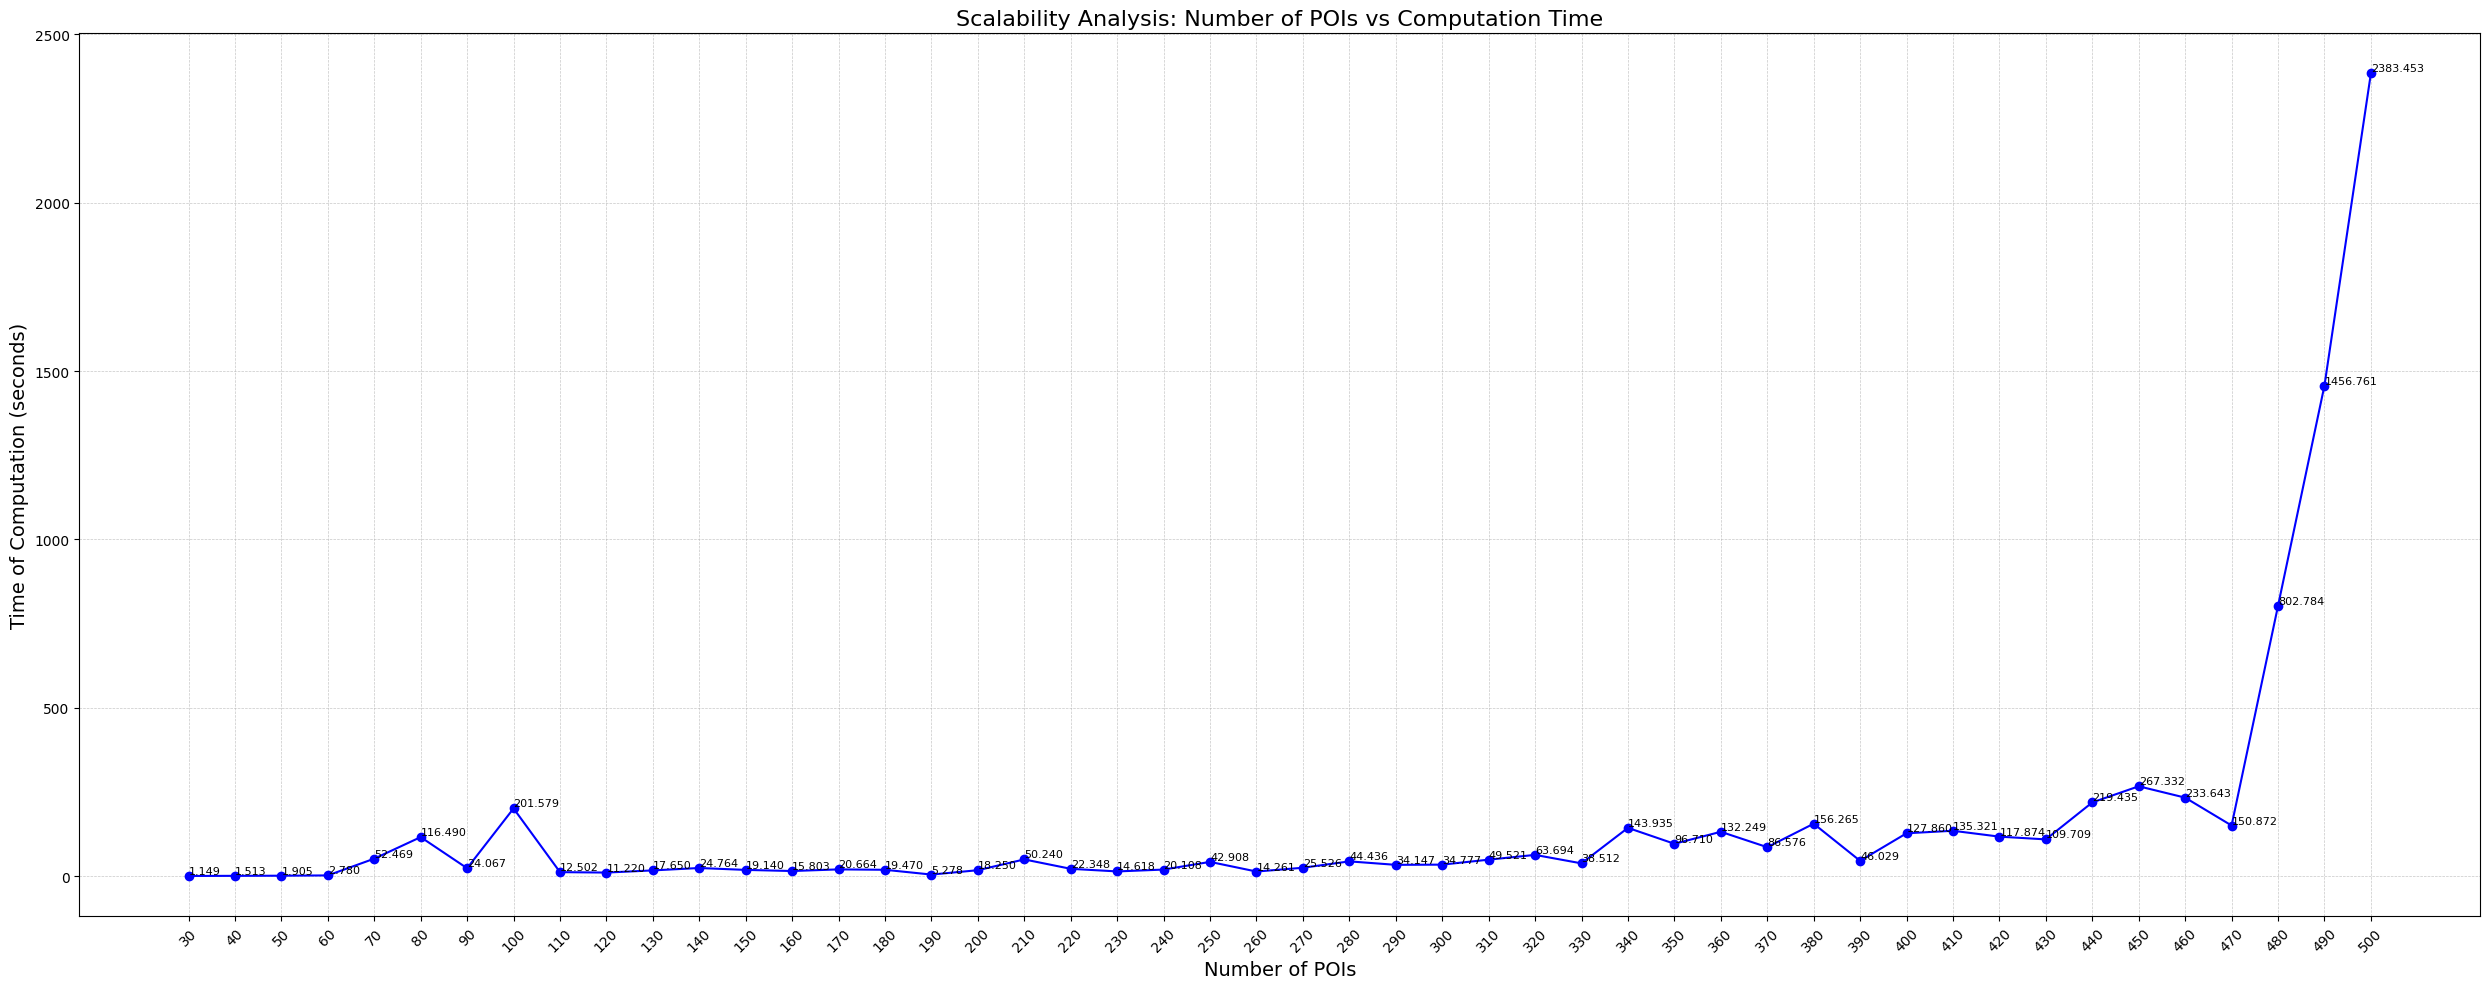
\includegraphics[width=\textwidth]{plots/scalability.png}
    \caption{Time of computation on increasing number of POIs in single-day trips.}
    \label{fig:scalability1}
\end{figure*}

Figure ~\ref{fig:dynamic} shows the effect of the dynamic nature of our itinerary planner,where we conducted an analysis based on three distinct user behavior scenarios. Our planner dynamically recalculates the itinerary by considering the actual time a user spends at each Point of Interest (POI) and the time taken to travel between them, in contrast to the initially suggested schedule. The three scenarios include: (1) \textit{30 Minutes Less Visiting Time}, where the user spends 30 minutes less at two POIs while keeping the travel time unchanged; (2) \textit{On time}, where the user follows the suggested visiting and travel times precisely; and (3) \textit{30 Minutes More Visiting Time}, where the user spends 30 minutes more at two POIs with the travel time remaining the same. As shown in figure, at a time budget of 480 minutes and cost budget of 8000 units in TRIP\_H\_B variant, the utility achieved in the first case is higher than the on-time scenario, while the utility in the third case is lower. This variation in utility values underscores the importance of adapting the itinerary based on real-time user behavior, demonstrating the effectiveness of our dynamically responsive planning approach.\\


\noindent\textbf{Scalability}\\
To evaluate the scalability of our itinerary planning system, we examine how the computation time required to generate a complete itinerary varies with the number of Points of Interest (POIs) in a city, while keeping the time and cost budgets fixed at sufficiently accommodating values of 600 minutes and 10000 units respectively. As illustrated in Figure~\ref{fig:scalability1}, the observed increase in computation time with the number of POIs is expected, given that our approach is formulated as an Integer Linear Program (ILP). This growth aligns with the theoretical complexity of the underlying problem — a variant of the Team Orienteering Problem — which is known to be NP-Hard. Despite this, our formulation remains tractable for problem sizes typical of real-world tourist cities. Despite this theoretical complexity, our system demonstrates strong practical performance. For instance, with approximately 270 POIs, the itinerary is generated in under 25 seconds. Even with nearly 430 POIs, the computation time remains under 110 seconds. These results highlight that, for realistically sized cities, our system maintains high computational efficiency, making it a viable and scalable solution for real-world deployment.

\begin{figure}[H]
    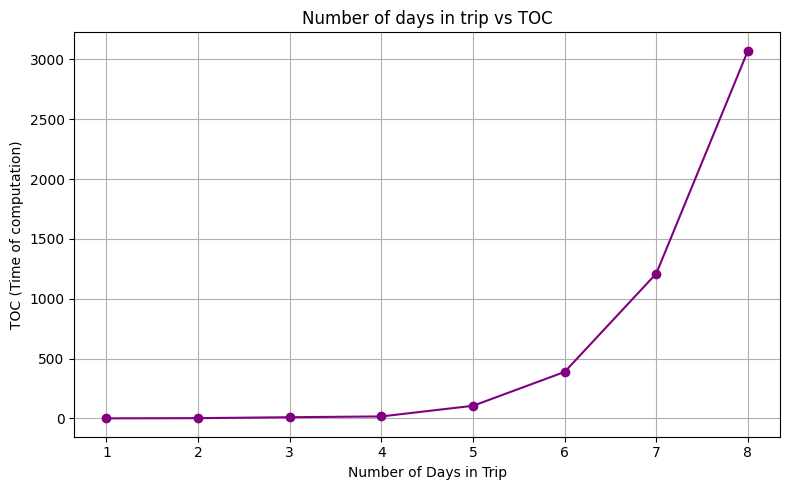
\includegraphics[width=0.4\textwidth]{plots/multidayVStoc.png}
     \caption{Time of computation on increasing number of days in multi-day trips}
    \label{fig:scalability2}
\end{figure}
We further analyze the scalability of our system by examining how the computation time varies with the number of days in the trip. As shown in Figure~\ref{fig:scalability2}, an increase in the number of days leads to a nonlinear growth in the time required to compute the optimal itinerary. This behavior is expected, as extending the trip duration increases the solution space exponentially due to the combinatorial nature of the underlying ILP formulation. Despite this, our system remains efficient for most practical use cases. For trips spanning up to 5 days, the computation time remains under 150 seconds, which is acceptable for interactive or semi-interactive planning scenarios. Even for longer trips (e.g., 7–8 days), where the computation time exceeds 1000 seconds, the planner still provides complete and optimized itineraries, reaffirming its robustness and practical viability for extended travel planning.
